\section{Passengers}

In this section the passengers of air traffic will be described. There will be looked at a survey conducted by eNT, to see how the passengers feel about the current air traffic.

When talking about air traffic it is of cause also very important to find out what the passengers themselves want, therefore this part of the report will look at what passengers think is the most important things for them in a flight.
In a survey made by eNT - Global Travel Industry News, they asked more than 3.200 people what they thought is the most important thing in their flight.
\begin{itemize}
\item 25\% - thought limited legroom was one of their biggest gripes about air travel
\item 30\% - lobbied for more legroom
\item 38\% - requested roomier seats
\item 25\% - consider airline fees to be their biggest complaint about air travel
\item 56\% - thought checked baggage fees were the most annoying current airline fee
\item 56\% - expect the overall cost of airline fees to rise in 2010
\item 74\% - think passengers of size should be required to purchase tickets for two seats on their flights
\item 21\% - think that airlines will add passenger of size fees in 2010
\item 30\% - they would be more likely to book a flight on an aircraft with in-flight Wi-Fi than one without
\item 61\% - they would not be willing to pay for in-flight Wi-Fi access
\item 27\% - they would be willing to pay \$5 or less for the service
\item If the person sitting next to them on their flight were accessing inappropriate content on their computer using in-flight Wi-Fi:
\begin{itemize}
\item 45\% - would do nothing
\item 27\% - would alert a flight attendant
\item 22\% - would ask their seatmate to close the inappropriate content
\item 6\% - would file a complaint with the airline
\end{itemize}
\item With the rise of checked baggage fees:
\begin{itemize}
\item 58\% - said they always or often carry on their bag to avoid extra charges, possibly adding to cramped overhead bins
\item 62\% - said they would put their carry-on bag above someone else's row if their own overhead space were already filled
\item 57\% - said that each seat on a plane should have assigned space in the overhead compartment, even if it meant carry-on bags had to be smaller
\end{itemize}
\item 79\% - said they are comfortable with U.S. airports using full body scanners that can see through clothes
\item 52\% - prefer the aisle seats
\item 44\% - favor the window seats
\item 33\% - request seats in the exit row on their flights
\item 13\% - ask for bulkhead seats
\item 39\% - cite long security lines as the most annoying part of being at an airport
\item 19\% - think that airports have high prices for food
\item 14\% - think that there is not enough seating in the boarding area
\item 95\% - think there should be a price limit on bottled water post-security at the airport, since security checkpoints require passengers to leave larger bottles behind
\end{itemize}

\subsection{Control during the journey [CHANGE!]}
Passengers want control over and knowledge about their journey on the run. A survey made by SITA (have no clue what it is a abbreviation for) in 2012 [http://www.sita.aero/content/airline-passengers-want-more-control] shows that 90\% of the 2,526 passengers included in the survey thinks that flight status updates on their mobile phones and self-boarding is their absolute top technologies when it comes to air travel. Furthermore an increasing rate of the world's population is getting smart phones and therefore also the rate of passengers. The number of passengers who has a smart phone went from 54\% in 2011 to 70\% in 2012 and is expected to reach 90\% in 2015. Therefore it it clear that the market for smart phone applications for the passengers witch can keep them informed about their flights, delays, boarding hours ect. and which they can also use to check-in and get their boarding passes from is something most airports and/or airlines should try to make. Already 21\% og passengers are now using mobile boarding pass.
Another survey made by IATA in 2012 shows that only a very small procentage uses the Airline application for smartphones to book their flight whereas 52\% books online via the airline website, see figure \ref{channes used to book}.

\begin{figure}
\centering
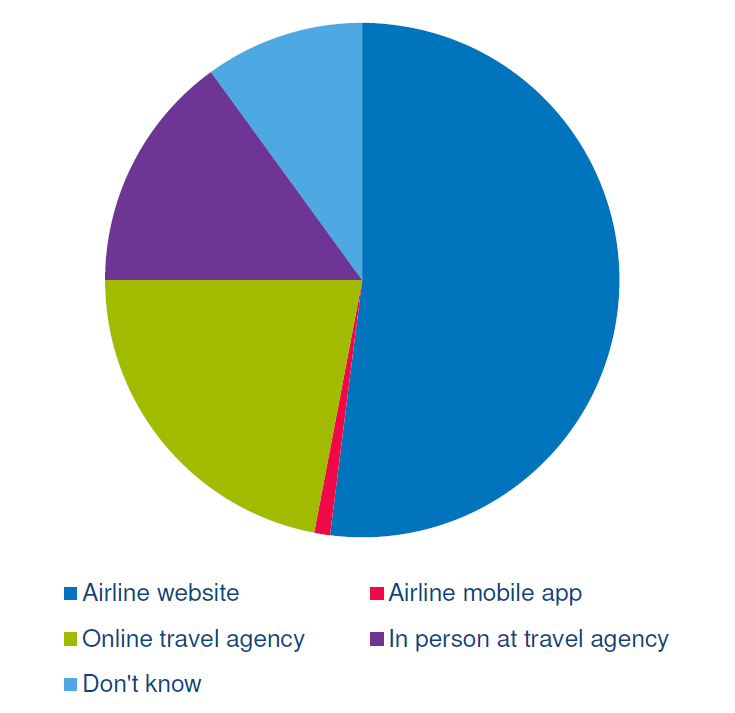
\includegraphics{Grafik/channes_used_to_book}
\caption{Breakdown of channels used to book flights.}
\label{channes used to book}
\end{figure}


In conclusion the passengers have different requirements for the companies, and it will not be easy to satisfy every customer fully. To do this would be a major challenge, but also one that might raise the number of people challenging with the air traffic.

%Kilder:
%http://www.iata.org/publications/Documents/2012-iata-global-passenger-survey-highlights.pdf
%http://business.time.com/2012/09/20/airline-introduces-perk-passengers-actually-want-and-its-free/
%http://consumertravelalliance.org/2011/02/06/what-do-airline-passengers-really-want-%E2%80%94-besides-a-good-fare/
%http://www.eturbonews.com/14902/survey-what-passengers-want-airlines
%http://elliott.org/blog/what-do-airline-passengers-really-want-besides-a-good-fare/
%http://blog.apex.aero/inflight-services-2/ten-premium-passengers-airlines/

